\section{Experiment Design and Methodology}\label{section:Experiment_Design_and_Methodology}
\subsection{Introduction}
As discussed in Chapter~\ref{production_of_random_binary_sequences}, the experimental design used in this study closely aligns with the methodology established by Nickerson and Butler~\cite{nickerson:2009}, serving as the foundational basis for this experiment. By adapting their established methodology to the current study and its novel application, this project not only compares the sequences generated by subjects with those expected from a random process according to the statistical definition, but also evaluates the predictability of each subject's responses using Prediction with Expert Advice and Vovk's Aggregating Algorithm~\cite{vovk:1990}. In theory, the more random a subject's sequence, the less predictable their responses, leading to greater losses for both the Learner and each of the relevant Experts.

\subsection{Experimental Design}
This chapter outlines the experimental design, which aims to assess how well individuals can generate random binary sequences when compared to theoretical randomness and their previous inputs. The study employs a within-subject design, where each participant is exposed to all conditions of the independent variable which, in his case, means they are required to repeat the generation process several times. This approach provides a comprehensive view of each individual's performance in generating random sequences.

The independent variable in this experiment is the method by which the participants generate their binary sequences, as each participant is allowed to enter their sequences independently of one another. The dependent variables include the frequencies of $0$s and $1$s in each sequence, the number and length of runs within each sequence, and the predictions generated by the Experts and the Learner, which will be discussed in further detail in the following sections. The control variables of this study include the instructions given to the subject before beginning the experiment, the length of each binary sequence inputted, and the total number of sequences entered. These control variables were devised with the intention of facilitating a more accurate comparison and analysis of the collected data between participants.

This study's subjects primarily consisted of postgraduate students from the Computer Science Department at Royal Holloway, University of London, with additional participants from the Psychology Department to create a more representative sample. Each sample was tasked with generating several 10-item sequences intended to mimic the results expected from a random process. These sequences were entered into a web application hosted on \href{https://arbarraclough.github.io/aggregating_algorithm/}{GitHub Pages}. Each 10-item sequence consisted of $0$s and $1$s (representing Heads and Tails) arranged in any order that the subject chose, and participants were allowed to enter the sequences at their own pace. Prior to beginning the experiment, subjects were presented with the following instructions on a modal screen shown upon loading the web page:

\begin{quote}
    \textit{Your task is to create a table of sequences each consisting of 10 items, either 0 or 1.}

    \textit{Imagine that several people have each tossed a fair coin 10 times and the results of their tosses are recorded in a table, with each row recording the outcomes of the 10 tosses by one person.}

    \textit{Your goal is to produce this table in such a way that if compared with a table of the results of actual coin tosses, it would not be possible to distinguish which table represented the actual coin tosses with statistical tests and which didn't.}
\end{quote}

Herein lies the first divergence from Nickerson and Butler's original design because the sequences entered by the subjects are always displayed and were concatenated into a single, continuous sequence (as shown in Figure 3), which is then passed to the Aggregating Algorithm as $\omega$s. In the original experiment, the sequence would only remain visible to the subject until they had entered 10 items, at which point it would disappear. The modification in this study allows the Aggregating Algorithm to better identify patterns in the user's inputs as an interval length of 10-bits would be insufficient in allowing the algorithm to determine which Experts should be given higher weighting in forming the Learner's predictions, thereby improving the learner's prediction accuracy. While the underlying algorithm treats the sequence differently to~\cite{nickerson:2009}, the sequences are still presented to the subject in 10-item chunks (as shown in Figure 4), consistent with the original method, to better align with the human short-term memory span of approximately 7 $\pm$ 2 items cited in~\ref{production_of_random_binary_sequences}. This chunking allows subjects to quickly review their previous inputs and continue generating sequences that they perceive as random.

\begin{figure}[h]
    \centering
    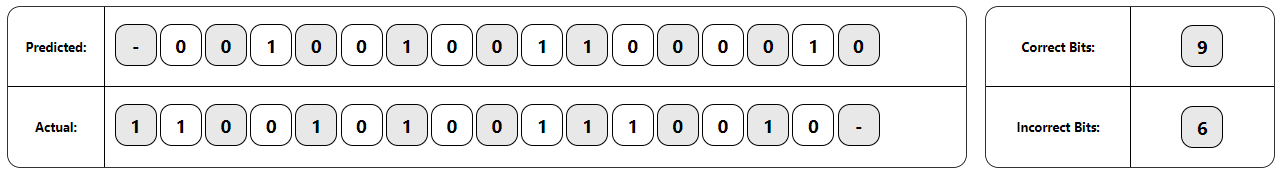
\includegraphics[width=0.9\textwidth]{images/sequence_input.png}
    \caption{Inputted Sequence Displayed in the Web Application}
\end{figure}

\begin{figure}[h]
    \centering
    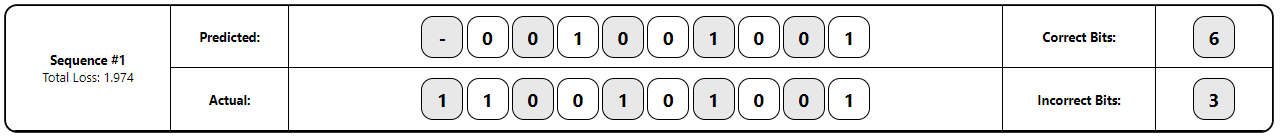
\includegraphics[width=0.9\textwidth]{images/past_sequences.png}
    \caption{Past Sequences Displayed in the Web Application.}
\end{figure}

Given this foundation, we can now discuss how the Aggregating Algorithm for Specialist Experts (AASE) was applied to this experiment.

\subsection{Applying the Aggregating Algorithm}
The Aggregating Algorithm, as well as the broader framework of Prediction with Expert Advice, are integral to this study. To apply these methods to this scenario, we must first define the $\eta$-mixable game $G = \langle \Gamma, \Omega, \lambda \rangle$, as defined in Protocol 2 \textendash{} Prediction with Expert Advice Framework. As suggested by Chapter 2, the primary focus of this project is Prediction with Expert Advice for the Discrete Binary Game which is formally defined by the triple consisting of the \textbf{\textit{outcome space}} $\Omega = \{0, 1\}$, the \textbf{\textit{prediction space}} $\Gamma = [0, 1]$, and the \textbf{\textit{loss function}} given by Brier's (or Square) Loss, $\lambda_\text{SQ}(\gamma_t, \omega_t) = {(\gamma_t - \omega_t)}^2$. In practical terms, this means that Nature generates binary outcomes, either $0$ or $1$, while both the Learner and the Experts predict values within the range $[0, 1]$.

With the game formally established, it is essential to define the roles of Nature, the Learner and the Experts in our experimental context. In this project, which assesses a subject's ability to generate random binary sequences, one of the key metrics is the predictability of their inputs prior to pressing a key. Therefore, each subject naturally assumes the role of Nature, while the Aggregating Algorithm functions as the Learner attempting to pre-empt Nature. As the experiment involves multiple subjects, this supports the assertion made previously that ``we make no assumptions about the outcome-generating mechanism (including the existence of such a mechanism).'' Each subject possesses a unique internal concept of randomness, and the Aggregating Algorithm must perform adequately across all participants and all sequences.

Finally, the concept of an Expert, as well as the rationale for making use of Specialist Experts and the Aggregating Algorithm for Specialist Experts, must also be defined. For our purposes, an Expert can be thought of as a function designed to predict the next outcome in a sequence based on the presence of a specific scenario. Since the experiment evaluates each subject's concept of randomness by statistically analysing conditional probabilities for different orders of dependency, it is natural to conceptualise the group of Experts as functions that search for specific prefixes within the sequence. As the subject inputs their sequence to the application, the last $n$ bits are passed to the group of Experts, who then assess whether the sequence currently falls within their ``area of expertise'', i.e., whether the last $n$ bits match the prefix that they are searching for.

Given that not every prefix will be relevant to each new subject input, the use of Specialist Experts is justified. If the current sequence does not match a Specialist's prefix, and thus ``area of expertise'', that Specialist is considered ``asleep'' and abstains from making a prediction, ``joining the crowd''. Conversely, Specialists whose prefixes match the sequence's ending are considered ``awake'' and make their predictions accordingly. It is important to note that there will never be a scenario where all Specialists are asleep, with at least one being awake at all timestamps, as there is always an Expert searching for the last $1\ -\ n$ bits of the sequence.

Finally, the details of how an Expert functions within this experiment must be explained. In order to generate the Experts, binary sequences up to length $5$ were generated and assigned to individual experts. The decision to limit the prefix length to 5-bits balances both computational efficiency with predictive accuracy, reflecting the established constraints of the human short-term memory typically spanning 7 $\pm$ 2 items. An Expert tracks the frequency of 0s and 1s following its specific prefix and makes predictions based on the ratio $\#1 / (\#0 + \#1)$. As subjects type their sequences, each Expert checks the last $x$ bits (corresponding to the length of their prefix) to determine whether they are awake. If so, the Specialist makes a prediction, which is then fed into the Aggregating Algorithm to inform the Learner's prediction for the next time stamp. For the sake of transparency, each Expert's last prediction, current prediction and status are displayed at the bottom of the application for user's reference if the subject is interested.

\subsection{Data Analysis}
After the experiment was conducted, the data was aggregated and analysed using various methods. The primary method was a chi-square goodness-of-fit test, comparing each subject's generated sequences to the distribution expected from a random process. To evaluate the Learner's performance, a secondary analysis was conducted, comparing both the cast (rounded) and uncast (unrounded) predictions against the actual outcomes.

Given the experiment involves playing Brier's Game with $\Omega = \{0, 1\}$ and $\Gamma = [0, 1]$, the simplest strategy for the Learner would be to predict $\nicefrac{1}{2}$ for every timestamp, which is the minimax prediction, resulting in a loss of $\nicefrac{1}{4}$ each time. Over 10 steps, the maximum loss for the Learner would be $\nicefrac{10}{4} = 2.5$, which serves as a benchmark for assessing the Aggregating Algorithm's performance \textendash{} loss less than $2.5$ indicates that a Learner using the Aggregating Algorithm predicts better than this naive strategy.

These methods of analysis are, in fact, somewhat adversarial, as the more statistically random a subject's input is, the more challenging it should become for the Experts, and thus the Learner, to make accurate predictions. Consequently, a better fit to statistical randomness should result in poorer Learner performance as the subject's sequences should exhibit no discernable patterns.

\subsection{Procedure}
This chapter outlines the step-by-step procedure followed to conduct the experiment based on what was outlined in the previous chapters.
\begin{enumerate}
    \item Participants were selected from the student community at Royal Holloway, University of London. Those recruited included postgraduate students from the Computer Science Department, as well as students from the Psychology Department, in order to create a diverse sample.
    \item Participants were directed to the application hosted on \href{https://arbarraclough.github.io/aggregating_algorithm/}{GitHub Pages} designed to collect and analyse generated binary sequences. Its development and the issues faced will be outlined in a following chapter.
    \item During the experiment, subjects were tasked with generating several 10-item binary sequences by entering 0s and 1s into the application such that the results would appear random if subjected to statistical tests. For transparency, the application displayed the internal workings of each Expert at the bottom of the screen, though participants could disable this feature if they desired.
    \item After finishing the experiment, the subjects were asked to email their results to \href{mailto:Andrew.Barraclough.2018@live.rhul.ac.uk}{Andrew.Barraclough.2018@live.rhul.ac.uk} to be subjected to the methods outlined in the previous section, namely chi-square goodness-of-fit and comparison to the loss inflicted by following the naive strategy.
\end{enumerate}